% Brian Mc George
% MCGBRI004
% 13/04/2015

\documentclass[]{article}
\title{Functional Programming Assignment 1\\Theoretical Questions}
\date{13-04-2015}
\author{Brian Mc George\\MCGRBRI004
}
\usepackage{graphicx}
\usepackage{amsfonts}
\usepackage{amsmath}
\usepackage{float}
\begin{document}

\maketitle
\newpage

\section*{Question 2.2}
The Rubik's cube can be twisted in six directions. For each state six new (non-distinct) states can be generated. \(n\) moves can be represented by the following mathematical function:
\begin{equation}\label{func_states}	
	f(n)=6^n\text{ for all }n \in\mathbb{N}
\end{equation}

\section*{Question 3.2}
Figure \ref{fig:memory_usage} indicates that there is a correlation between the running time and the memory usage. As \(n\) increases, so does the size of the search space grow exponentially. However, in terms of actually memory usage on the operating system we do not see this exponential growth, we instead see a logarithmic increase in memory usage of the process over the run duration.
% Memory Usage Image
\begin{figure}[H]
\centering
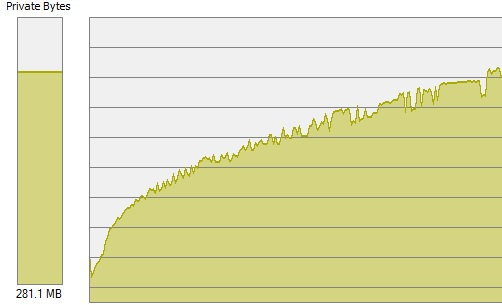
\includegraphics[width=1\linewidth]{memory_usage.jpg}
\caption{Memory Usage Over Time}
\label{fig:memory_usage}
\end{figure}
\begin{table}[H]
\begin{center}
	\begin{tabular}{|r|c|l|}
		\hline
		Size of \(n\)&Peak Memory Usage (MB)&Running Time (Seconds)\\
		\hline
		1&n/a&0.047\\
		2&n/a&0.049\\
		3&n/a&0.055\\
		4&n/a&0.098\\
		5&n/a&0.355\\
		6&53.9&7.034\\
		7&273.2&213.197\\
		8&null&null\\
		\hline
		
	\end{tabular}\caption{Memory usage and running time for different size of \(n\)}\end{center}
	\label{table:mem_usage}
\end{table}

Tests were conducted for \(n\) up to size 8. The results would indicate ...

\section*{Question 4}
Using function \ref{func_states}, the number of states that can be generated from 10 moves where 6 possible rotations can be made for each state is
\begin{equation*}
\begin{split}
  f(10) & = 6^{10} \\
		  & = 60466176\text{ states}
\end{split}
\end{equation*}								
Function \ref{func_states} can be optimised such that from a given non-initial state, the new states generated are only those that will not undo the last move.
\begin{equation}
\begin{split}
f(n) =
\begin{cases}
	6^{n} & \text{if }n \in T = \{0, 1\}\\
	5^{n} & \text{if }n \in \mathbb{N} \setminus T\\
	0 & \text{otherwise}
\end{cases}
\end{split}
\end{equation}	


\end{document}
